\xiti
\begin{xiaotis}

\xiaoti{求棱长为 $a$ 的正八面体的对角线长。}

\xiaoti{以正四面体的高和棱为一边分别作正方形。求证:这两个正方形的面积比是 $2:3$。}

\xiaoti{正六面体各面中心是一个正八面体的顶点。求这个正六面体和正八面体的表面积的比。}

\xiaoti{正 $n$ ($n = 4$,$8$,$20$)面体的棱长为 $a$。求它们表面积的共同公式。}

\xiaoti{正二十面体的棱长为 $a$,连结相对顶点的对角线为 $b$,求它的体积。}

\xiaoti{求证:平行于正四面体的相对棱的平面,截这个正四面体的截面是一个矩形。}

\xiaoti{就下面平面图形验证 $V + F - E = 1$。}

\begin{figure}[htbp]
    \centering
    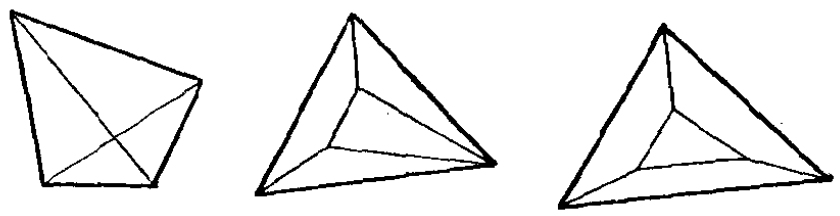
\includegraphics[width=8cm]{../pic/ltjh-ch3-xiti17-07.png}
    \caption*{(第 7 题)}
\end{figure}

\xiaoti{已知:凸多面体的各面都是四边形,求证:$F = V - 2$。}

\end{xiaotis}

